\chapter{Introduction}
The idea that we learn by interacting with our environment is probably the first to occur.
to us when we think about the nature of learning. When an infant plays, waves its arms,
or looks about, it has no explicit teacher, but it does have a direct sensorimotor connection.
to its environment. Exercising this connection produces a wealth of information about
cause and effect, about the consequences of actions, and about what to do to achieve goals. Throughout our lives, such interactions are undoubtedly a major source. of knowledge about our environment and ourselves. Whether we are learning to drive a car or to hold a conversation, we are acutely aware of how our environment responds. to what we do, and we seek to influence what happens through our behavior. Learning from interaction is a foundational idea underlying nearly all theories of learning and intelligence.

\section{Reinforcement Learning}
\subsection{Meaning}
Reinforcement learning is learning what to do think in other way how to behave in such situations to make some reaction or as in literature action to certain state you are in 
as to maximize a numerical reward signal. The learner is not told how to behave or which action he must take but he discovers it with trial and error and decide which action achieve the highest reward which map to the best action reward but also the next situation and, through that, all subsequent rewards. These two characteristics—trial-and-error search and delayed reward—are the two most important distinguishing features of reinforcement learning.
The basic idea is simply to capture the most important aspects of the real problem facing a learning agent interacting over time with its environment to achieve a goal. A learning agent
must be able to sense the state of its environment to some extent and must be able to
take actions that affect the state. The agent also must have a goal or goals relating to
the state of the environment. Markov decision processes are intended to include just.
these three aspects—sensation, action, and goal—in their simplest possible forms without
trivializing any of them. Any method that is well suited to solving such problems we
consider to be a reinforcement learning method.

\subsection{RL \& Machine Learning}
Reinforcement learning is also different from what machine learning researchers call. 
Unsupervised learning, which is typically about finding structure hidden in collections of
unlabelled data. The terms supervised learning and unsupervised learning would seem.
to exhaustively classify machine learning paradigms, but they do not. Although one
might be tempted to think of reinforcement learning as a kind of unsupervised learning.
because it does not rely on examples of correct behavior, reinforcement learning is trying.
to maximize a reward signal instead of trying to find hidden structure.\\
Uncovering structure in an agent's experience can certainly be useful in reinforcement learning,
but by itself does not address the reinforcement learning problem of maximizing a reward signal.
We therefore consider reinforcement learning to be a third machine learning paradigm,
alongside supervised learning and unsupervised learning and perhaps other paradigms. 

\begin{wrapfigure}{h}{0.4\textwidth}
    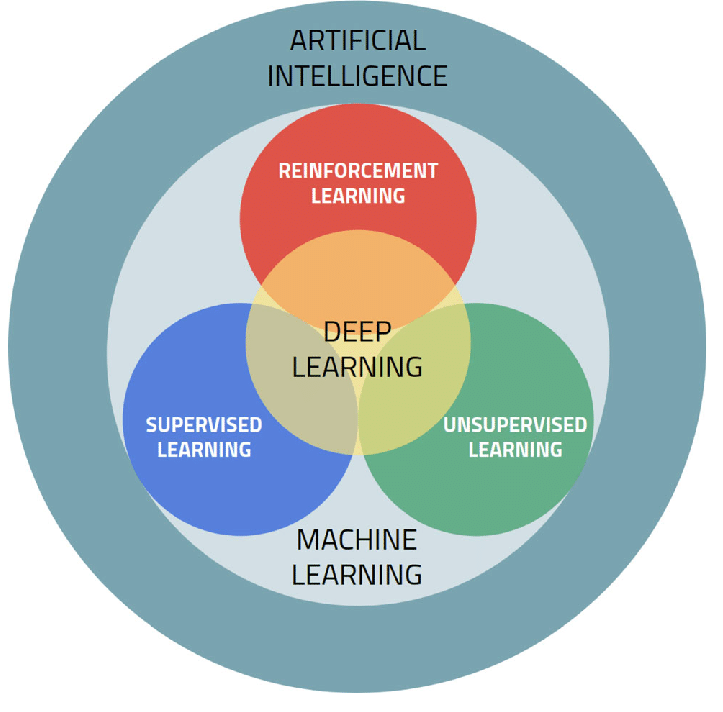
\includegraphics[width=0.4\textwidth]{35.PNG}
  \caption{Artificial Intelligence Map}
\end{wrapfigure}

One of the challenges that arise in reinforcement learning, and not in other kinds.
of learning, is the trade-of between exploration and exploitation. To obtain a lot of
reward, a reinforcement learning agent must prefer actions that it has tried in the past.
and found to be effective in producing reward. But to discover such actions, it must
try actions that it has not selected before. The agent must exploit what it has already.
experienced in order to obtain reward, but it also has to explore in order to make better.
action selections in the future. The dilemma is that neither exploration nor exploitation.
can be pursued exclusively without failing at the task. The agent must try a variety of
actions and progressively Favor those that appear to be best. On a stochastic task, each
action must be tried many times to gain a reliable estimate of its expected reward. The
exploration-exploitation dilemma has been intensively studied by mathematicians for
many decades yet remains unresolved. For now, we simply note that the entire issue of
balancing exploration and exploitation do not even arise in supervised and unsupervised.
learning, at least in the purest forms of these paradigms.
Another key feature of reinforcement learning is that it explicitly considers the whole.
problem of a goal-directed agent interacting with an uncertain environment. This is in
contrast to many approaches that consider sub-problems without addressing how they
might fit into a larger picture. 

Reinforcement learning takes the opposite tack, starting with a complete, interactive,
goal-seeking agent. All reinforcement learning agents have explicit goals, can sense.
aspects of their environments and can choose actions to influence their environments.
Moreover, it is usually assumed from the beginning that the agent must operate despite
significant uncertainty about the environment it faces. When reinforcement learning
involves planning, it must address the interplay between planning and real-time action.
selection, as well as the question of how environment models are acquired and improved.
When reinforcement learning involves supervised learning, it does so for specific reasons.
that determine which capabilities are critical and which are not. For learning research to
make progress, important sub-problems must be isolated and studied, but they should.
be sub-problems that play clear roles in complete, interactive, goal-seeking agents, 
even if all the details of the complete agent cannot yet be filled in.
By a complete, interactive, goal-seeking agent we do not always mean something like
a complete organism or robot. These are clearly examples, but a complete, interactive,
goal-seeking agent can also be a component of a larger behaving system. In this case,
the agent directly interacts with the rest of the larger system and indirectly interacts.
with the larger system's environment. 

One of the most exciting aspects of modern reinforcement learning is its substantive.
and fruitful interactions with other engineering and scientific disciplines. 
Reinforcement learning is part of a decades-long trend within artificial intelligence and machine learning toward greater integration with statistics, optimization, and other mathematical subjects.
Of all the forms of machine learning, reinforcement learning is the closest to the kind of learning that humans and other animals do, and many of the core algorithms of reinforcement
learning was originally inspired by biological learning systems. Reinforcement learning
has also given back, both through a psychological model of animal learning that better
matches some of the empirical data, and through an influential model of parts of the
brain's reward system. The body of this book develops the ideas of reinforcement learning.
that pertain to engineering and artificial intelligence, with connections to psychology and
neuroscience.

\subsection{Vocabulary of Reinforcement Learning}
Beyond the agent and the environment, one can identify \emph{four main sub-elements} of any reinforcement learning system:
\begin{description}
    \item[A policy:] A policy defines \emph{the learning agent's way of behaving at a given time}. Roughly speaking, a policy is a mapping from perceived states of the environment to actions to be taken when in those states.
    \item[Reward signal (the goal of RL):] A reward signal defines \emph{the goal} of a reinforcement learning problem. On each time step, the environment sends to the reinforcement learning agent a single number called the reward. The agent's sole objective is to maximize the total reward it receives over the long run. The reward signal thus defines what are the good and bad events for the agent.
    \item[Value function:] A value function specifies \emph{what is good in the long run}. Roughly speaking, the value of a state is the total amount of reward an agent can expect to accumulate over the future, starting from that state to the end. A state might always yield a low immediate reward but still have a high value because it is regularly followed by other states that yield high rewards.
    \item[Model of the environment:] This is \emph{something that mimics the behavior of the environment}, or more generally, that allows inferences to be made about how the environment will behave.
\end{description}

\section{An Example: Tic-Tac-Toe}
Consider the familiar child's game of tic-tac-toe (Figure~\ref{fig:tic-tac-toe}). Two players take turns playing on a three-by-three board. One player plays Xs and the other Os until one player wins by placing three marks in a row, horizontally, vertically, or diagonally.
If the board fills up with neither player getting three in a row, then the game is a draw like illustrated in Figure~\ref{fig:tic-tac-toe}. Because a skilled player can play so as never to lose, let us assume that we are playing against an imperfect player, one whose play is sometimes incorrect and allows us to win. 
For the moment, in fact, let us consider draws and losses to be equally bad for us. \\
Now the question is: \textbf{How might we construct a player that will find the imperfections in its opponent's play and learn to maximize its
chances of winning?}

\begin{wrapfigure}{h}{0.4\textwidth}
    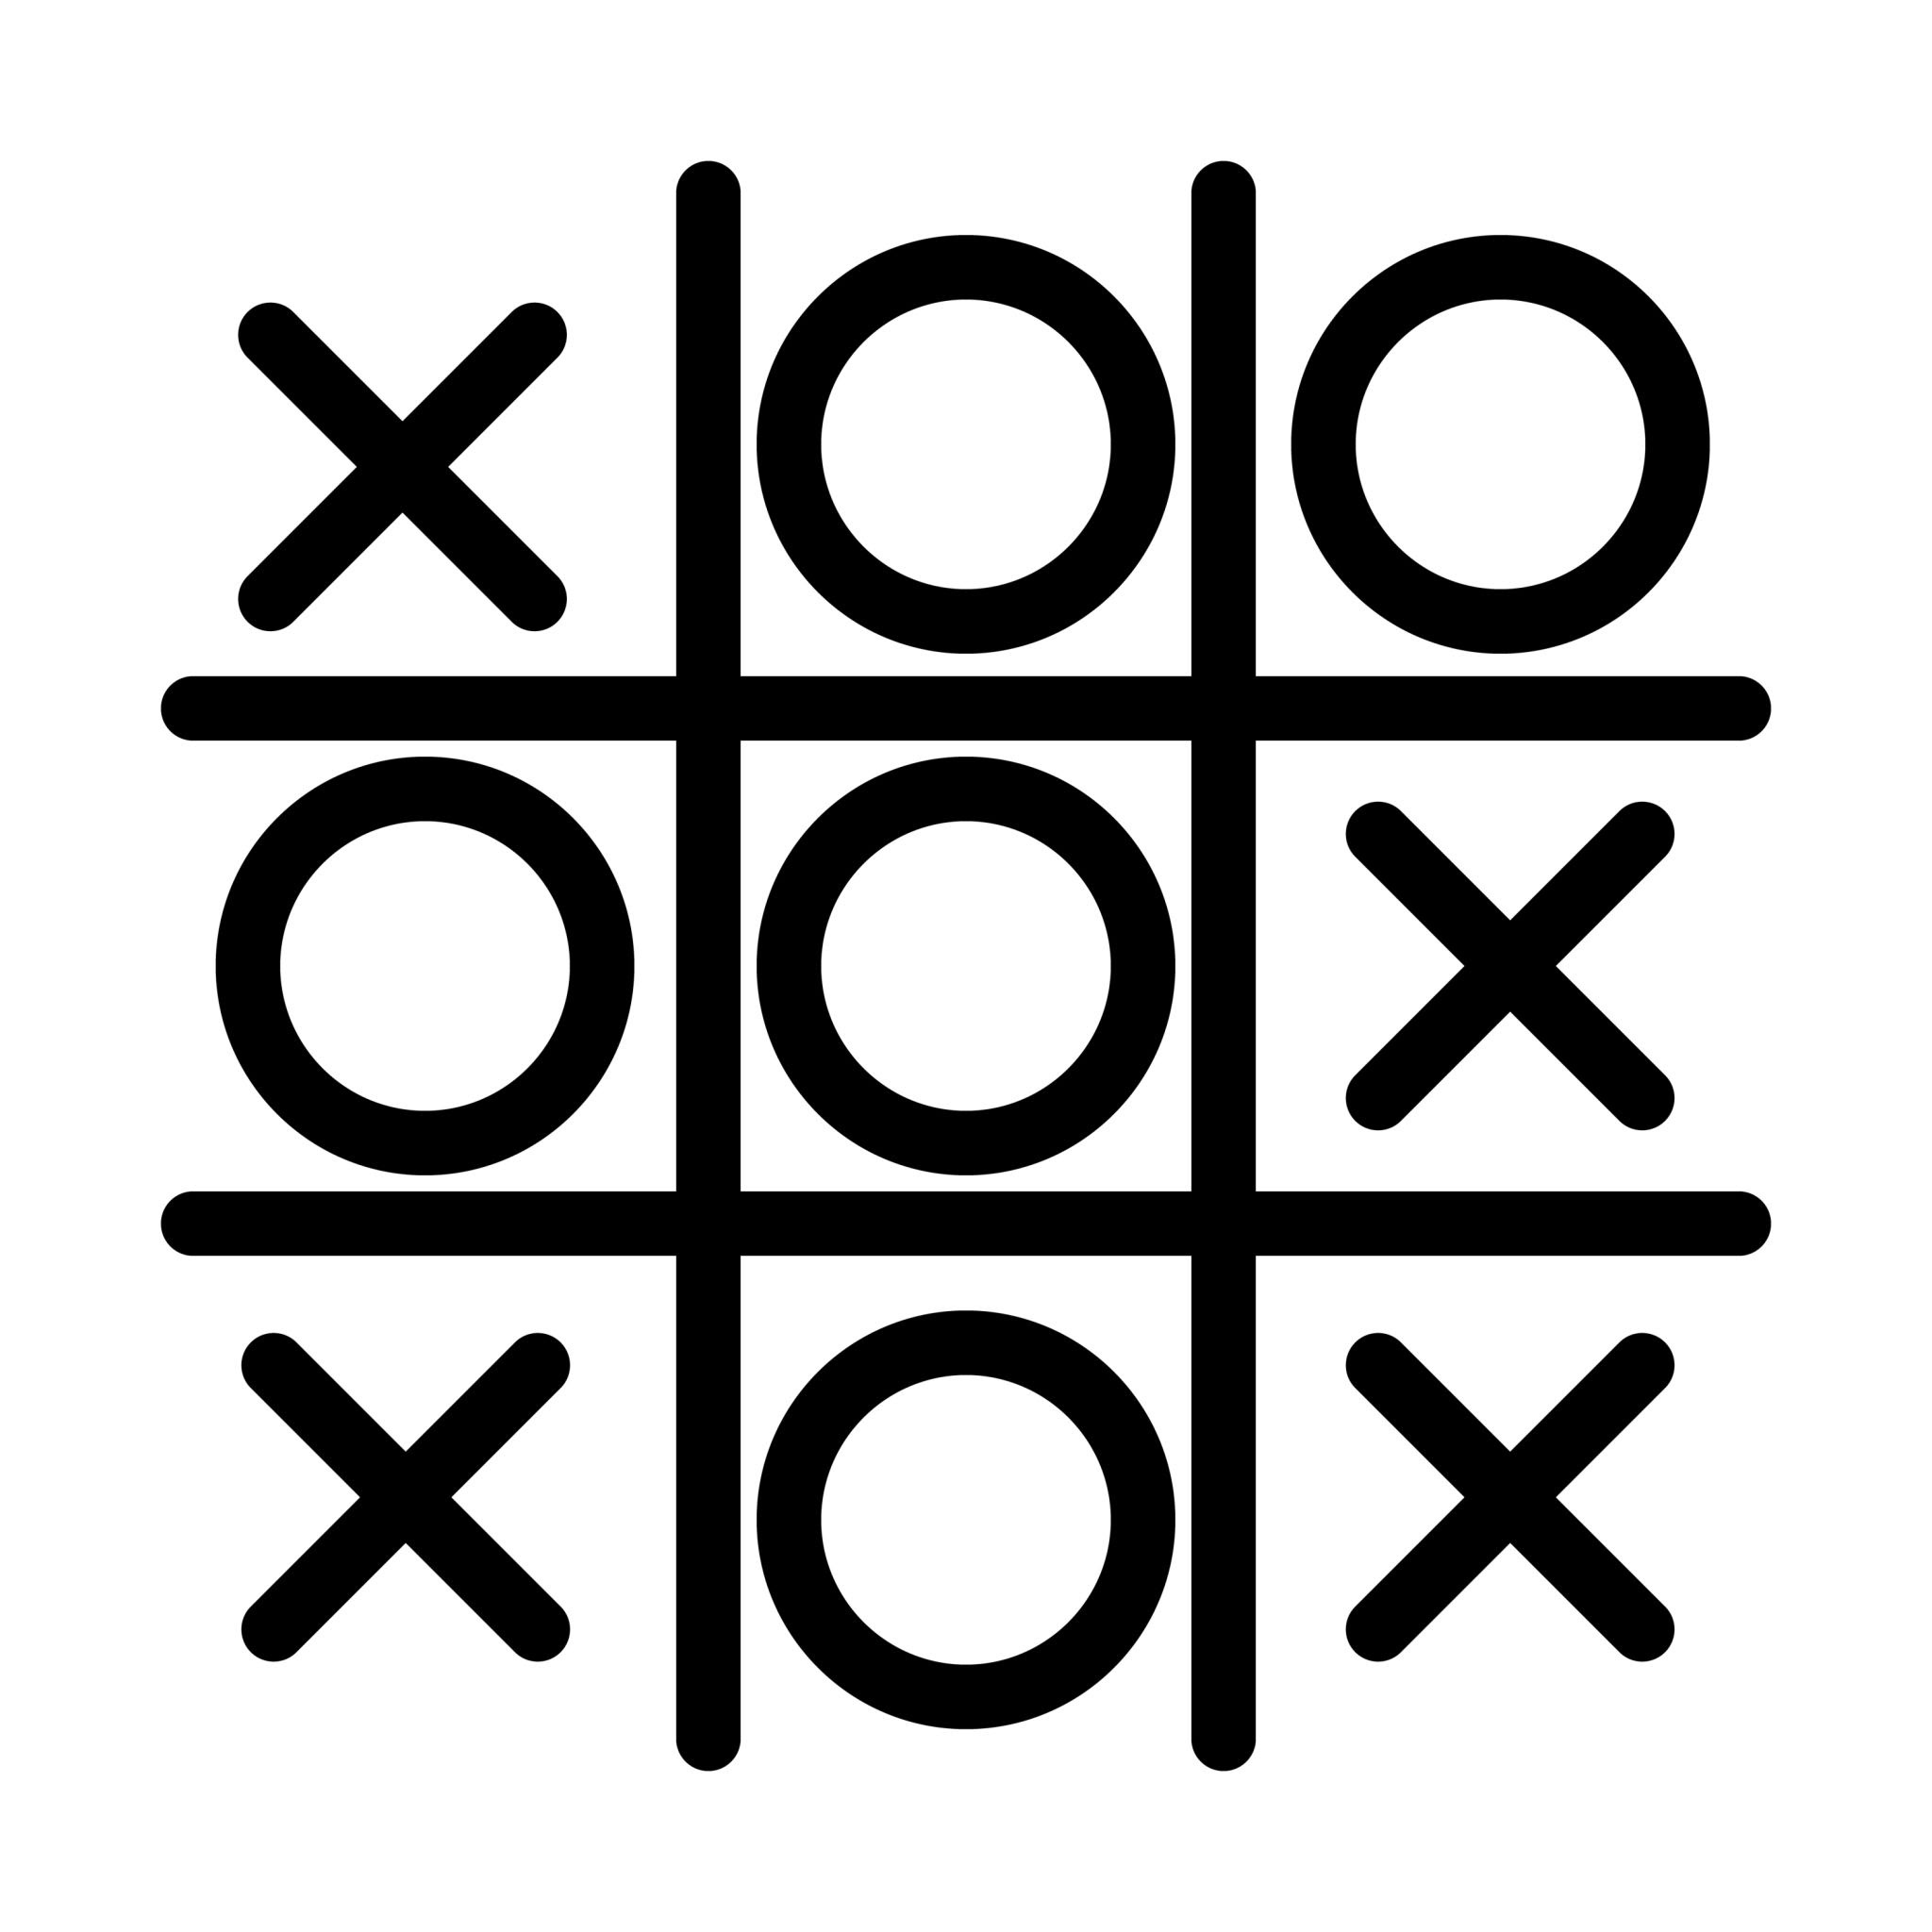
\includegraphics[width=0.4\textwidth]{36.jpeg}
  \caption{Tic-Tac-Toe}
  \label{fig:tic-tac-toe}
\end{wrapfigure}

\emph{Classical optimization methods} for sequential decision problems, such as dynamic programming, can compute an optimal solution for any opponent, but require as input a complete specification of that opponent, including the probabilities with which he opponent makes each move in each board state. 
Let us assume that this information is not available a priori for this problem, as it is not for
most problems of practical interest. On the other hand, such information can be estimated from experience, in this case by playing many games against the opponent. About the best one can do on this problem is first to learn a model of the opponent's behavior, up to some level of
confidence, and then apply dynamic programming to compute an optimal solution given
the approximate opponent model. \\
\emph{An evolutionary method }applied to this problem would directly search the space
of possible policies for one with a high probability of winning against the opponent.
Here, a policy is a rule that tells the player what move to make for every state of the
game—every possible configuration of Xs and Os on the three-by-three board. For each
policy considered, an estimate of its winning probability would be obtained by playing
some number of games against the opponent. This evaluation would then direct which
policy or policies were considered next. A typical evolutionary method would hill-climb
in policy space, successively generating and evaluating policies in an attempt to obtain
incremental improvements. Or, perhaps, a genetic-style algorithm could be used that
would maintain and evaluate a population of policies. Literally hundreds of different
optimization methods could be applied. \\

\begin{wrapfigure}{l}{0.4\textwidth}
    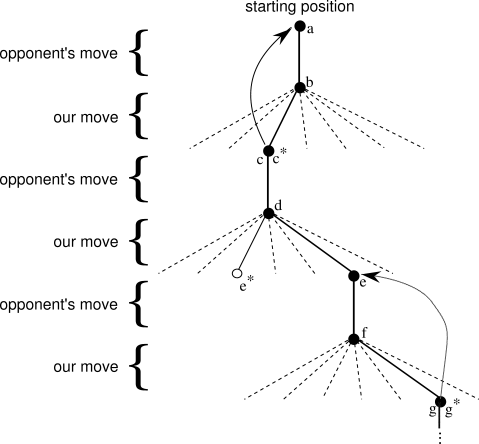
\includegraphics[width=0.4\textwidth]{37.PNG}
  \caption{A sequence of tic-tac-toe moves.}
  \label{fig:tic-tac-toe moves}
\end{wrapfigure}

Here is how the tic-tac-toe problem would be approached with a method making use of a value function: \\
\textbf{First,} we would set up a table of numbers, one for each possible state
of the game. Each number will be the latest estimate of the probability of our winning.
from that state. We treat this estimate as the state's value, and the whole table is the
learned value function. State A has higher value than state B or is considered “better”.
than state B, if the current estimate of the probability of our winning from A is higher.
than it is from B. Assuming we always play Xs, then for all states with three Xs in a row
the probability of winning is 1, because we have already won. Similarly, for all states
with three Os in a row, or that are filled up, the correct probability is 0, as we cannot.
win from them. We set the initial values of all the other states to 0.5, representing a
guess that we have a 50\% chance of winning. \\
\textbf{Then,} we play many games against the opponent. To select our moves, we examine the 
states that would result from each of our possible moves (one for each blank space on the
board) and look up their current values in the table. Most of the time we move greedily,
selecting the move that leads to the state with greatest value, that is, with the highest. estimated probability of winning. Occasionally, however, we select randomly from among
the other moves instead. These are called exploratory moves because they cause us to
experience states that we might otherwise never see. A sequence of moves made and
considered during a game can be diagrammed as in the Figure~\ref{fig:tic-tac-toe moves}. \\
While we are playing, we change the values of the states in which we find ourselves.
during the game. We attempt to make them more accurate estimates of the probabilities.
of winning. To do this, we “back up” the value of the state after each greedy move to
the state before the move, as suggested by the arrows in Figure~\ref{fig:tic-tac-toe moves}. More precisely, the
current value of the earlier state is updated to be closer to the value of the later state.
This can be done by moving the earlier state's value a fraction of the way toward the
value of the later state. If we let $\mathbf{S}_t$ denote the state before the greedy move, and $\mathbf{S}_{t + 1}$
the state after the move, then the update to the estimated value of $\mathbf{S}_t$, denoted $\mathbf{V}\left(\mathbf{S}_t\right)$,
can be written as
\[ \mathbf{V}\left( \mathbf{S}_t \right) \leftarrow \mathbf{V}\left( \mathbf{S}_t \right) + \alpha \left[ \mathbf{V}\left( \mathbf{S}_{t+1} \right) - \mathbf{V}\left( \mathbf{S}_t \right) \right] \]
here $\alpha$ is a small positive fraction called \emph{the step-size parameter}, which influences 
the rate of learning. This update rule is an example of a temporal-difference learning.
method, so called because its changes are based on a difference, $\mathbf{V}\left( \mathbf{S}_{t+1} \right) - \mathbf{V}\left( \mathbf{S}_t \right)$ between
estimates at two successive times.

\section{Problem Formulation}
\subsection{Reinforcement Learning Taxonomy}
\begin{figure}[ht]
    \centering
    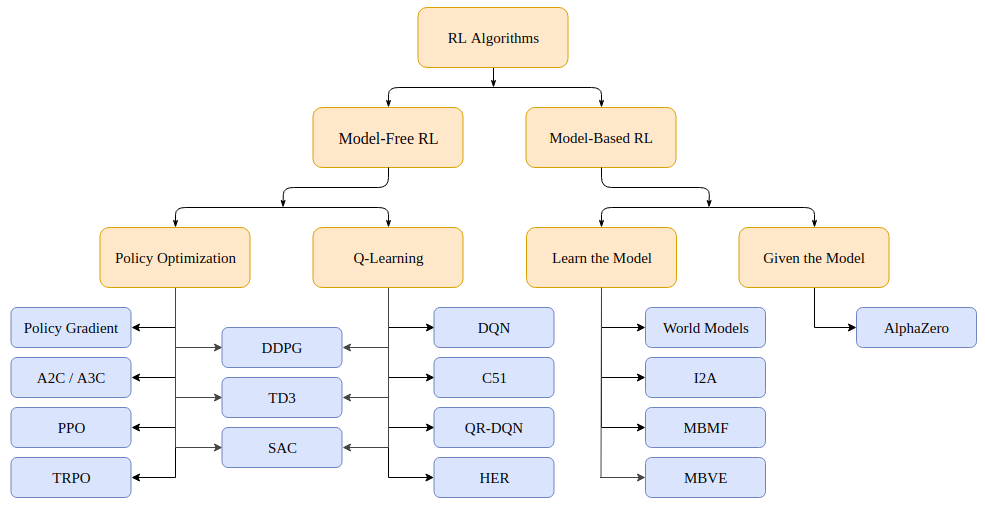
\includegraphics[width=0.7\textwidth]{38.PNG}
    \caption{RL Taxonomy}
    \label{fig:RL Taxonomy}
\end{figure}

\subsection{Problem Nature}
\subsubsection{Continuous or Discrete}
We have found that our problem has a \emph{Continuous action and state space} since in a real-world situation, the states space is mostly continuous, with uncountable states and actions combinations for an agent to explore and in our problem the channel has infinite changes so it can have infinite number of pre-coders for each of these states.
So we have excluded algorithms which depend on discrete spaces.

\subsubsection{Deterministic or Stochastic}
In AI and Reinforcement Learning (RL), policy refers to an agent's strategy to interact with an environment. Policies define the behavior of an agent. A policy determines the next action an agent takes in response to the current state of the environment. 
In other words, A policy is a function that maps a state to an action. Depending on the context and problem at hand, policies can be deterministic or stochastic. In this tutorial, we explain the difference between these two policy types.
\begin{figure}[ht]
    \centering
    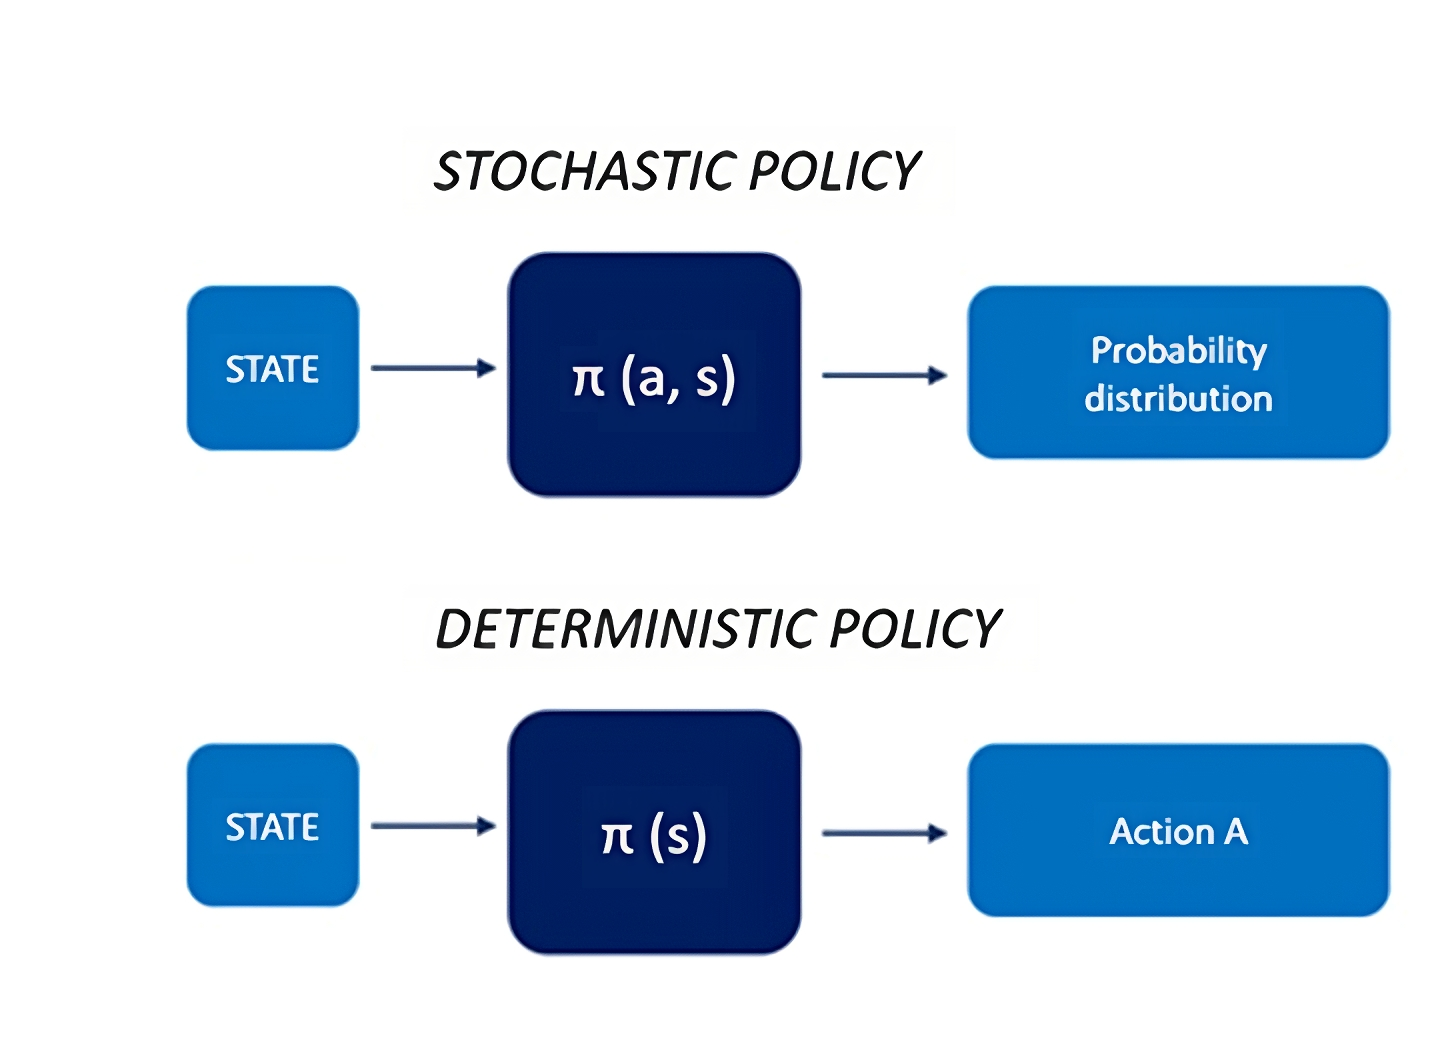
\includegraphics[width=0.4\textwidth]{39.PNG}
    \caption{Deterministic vs. Stochastic Policies}
    \label{fig:Deterministic vs. Stochastic Policies}
\end{figure}

\begin{description}
    \item[Deterministic Policy:] A deterministic policy is a policy that maps each state to a single action with certainty. In other words, the agent will always take the same action given a state. This policy is represented by a function $\pi : \mathbf{S} \rightarrow \mathbf{A}$ where $\mathbf{S}$ is the state space, and $\mathbf{A}$ is the action space. The deterministic policy function maps each state $s \in \mathbf{S}$ to a single action $a \in \mathbf{A}$.
    The advantage of a deterministic policy is that it is easy to interpret and implement. It is also suitable for tasks where the same action should be taken for the same state every time. \textit{For example}, in a chess game, the best move for a given board configuration is always the same. A deterministic policy can be the best choice to play the game optimally in such cases.    
    \item[Stochastic Policy:] A stochastic policy is a policy that maps each state to a probability distribution over actions. In other words, given a state, the agent will choose an action randomly based on the probability distribution. We represent this policy by a function $\pi : \mathbf{S} \times \mathbf{A} \rightarrow [0, 1]$ where $\mathbf{S}$ is the state space, $\mathbf{A}$ is the action space, and $\pi \in (s,a)$ is the probability of taking an action $a$ in a state $s$.
    The advantage of a stochastic policy is that it can capture the uncertainty in the environment. \textit{For example,} in a poker game, the agent may not always take the same action in response to the same hand since there is a probability of winning or losing depending on the opponent's hand and how the betting has proceeded. In such cases, a stochastic policy learns the best strategy based on the probability of winning.    
\end{description}

\textbf{Comparison}\\
The primary difference between a deterministic and stochastic policy is the way in which they choose actions. A deterministic policy chooses a single action for each state, while a stochastic policy chooses from a probability distribution over actions for each state. This means that a deterministic policy always chooses the same action for the same state, while a stochastic policy may choose different actions for the same state.
So depending on our problem nature where we need an exact pre-coder which will be optimal for a channel space so we need to have deterministic policy which leads to exclude some algorithms.

\subsection{Model Nature}
We interact with the environment all the time. Every decision we make influences our next ones in some unknown way. This behavior is the core of Reinforcement Learning (RL), where instead the rules of interaction and influence are not unknown, but predefined. RL algorithms can be either Model-free (MF) or Model-based (MB). If the agent can learn by making predictions about the consequences of its actions, then it is MB. If it can only learn through experience, then it is MF.
In Reinforcement Learning, we have an agent which can take action in an environment. Additionally, there are probabilities associated with transitioning from one environment state to another. These transitions can be deterministic or stochastic.
Ultimately, the goal of RL is for the agent to learn how to navigate the environment to maximize a cumulative reward metric.

\subsubsection{Model-Free RL}
\begin{wrapfigure}{r}{0.22\textwidth}
    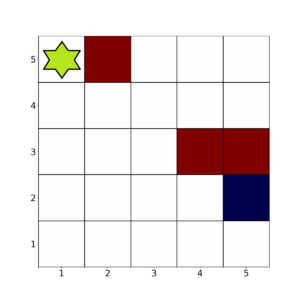
\includegraphics[width=0.22\textwidth]{40.PNG}
  \caption{5x5 environment}
  \label{fig:5x5 environment}
\end{wrapfigure}
Simply put, model-free algorithms refine their policy based on the consequences of their actions.as an example! \\
Consider this $5\times5$ environment (Figure~\ref{fig:5x5 environment})\\
In this example, we want the agent (in green) to avoid the red squares and reach the blue one in as few steps as possible.
To achieve this, we need to define an appropriate reward function. Here's one way:
\begin{itemize}
    \item Landing on an empty square: -1 point
    \item Landing on a red square: -100 points
    \item Landing on the blue square: +100 points
\end{itemize}
The agent has 4 possible actions: left, right, up, and down. On the edges, it has only 2 or 3 of these choices.

\subsubsection{Model-Based RL}
In a way, we could argue that Q-learning is model-based. After all, we are building a Q-table, which can be seen as a model of the environment. However, this is not how the term model-based is used in the field.
To classify as model-based, the agent must go beyond implementing a model of the environment. That is, the agent needs to make predictions of the possible rewards associated with certain actions.
This provides many benefits. For example, the agent interacts with the environment a few times. Then, the model uses this information to simulate subsequent iterations without needing to interact with the environment.
Using supervised learning, we can optimize the model to determine which trajectories are most likely to generate the biggest rewards.

\subsection{Policy Learning Type}
\subsubsection{ON Policy}
In on policy learning the agent learns about the policy used to generate the data. It means to learn about a policy. We simply mean learning the value function and in control We mean learning the optimal policy.
\subsubsection{OFF Policy}
In off policy learning the agent learns about a policy from data generated by following a different policy. That is the policy that we are learning is off the policy. They we are using for Action selection. \\

For example, you could learn the optimal policy while following a totally random policy we call the policy that the agent is learning the target policy because it is the target of the agents learning the target policy is usually denoted by $\pi$. The value function that the agent is learning is based on the target policy one example of a Target policy is the optimal policy we call the policy that the agent is using to select actions the behavior policy because it defines our agents behavior. 
The behavior policy is usually denoted by b. The behavior policy is in charge of selecting actions for the agent, so we are coupling the behavior from the target policy Because it provides another strategy for continual exploration. If our agent behaves according to the Target policy, it might only experience a small number of states. If our agent can behave according to a policy that favors exploration. It can experience a much larger number of states. 
Another key rule of off policy learning is that the behavior policy must cover the target policy In other words, if the target policy says the probability of selecting an action a given State s is greater than zero then the behavior policy must say the probability of selecting that action in that state is greater than 0 .It's worth noting that off policy learning is a strict generalization of on policy learning on policies the specific case where the target policy is equal to the behavior policy.

\subsection{Types of RL Gradients}
\begin{description}
    \item[Value-Based:] learn the state or state-action value. Act by choosing the best action in the state. Exploration is necessary.
    \item[Policy-Based:] Directly learn the stochastic policy function that maps state to action. Act by sampling policy.
    \item[Model-Based:] learn the model of the world, then plan using the model. Update and re-plan the model often.
\end{description}

We now focus on the policy gradient algorithms which learn a stochastic policy to maximize a cumulative reward.
However, they can suffer from high variance, slow convergence, and poor exploration but we need add judgment or criticism to our action to be sure it is the best which need to add value-based gradient to determine if the action is the best. \\

Eventually this led us to ACTOR-CRITIC algorithms. Actor-critic algorithms are a variant of policy gradient methods that use an additional value function, called the critic, to reduce the variance of the policy gradient and improve the learning efficiency, and to add the determinism to our model we have especially chosen DDPG algorithm (discussed in the next chapter).
